\newSec[Arch]{Software-Architektur}{1}




\begin{figure}[ht!]
\vspace{0.25cm}
\begin{center}
\fbox{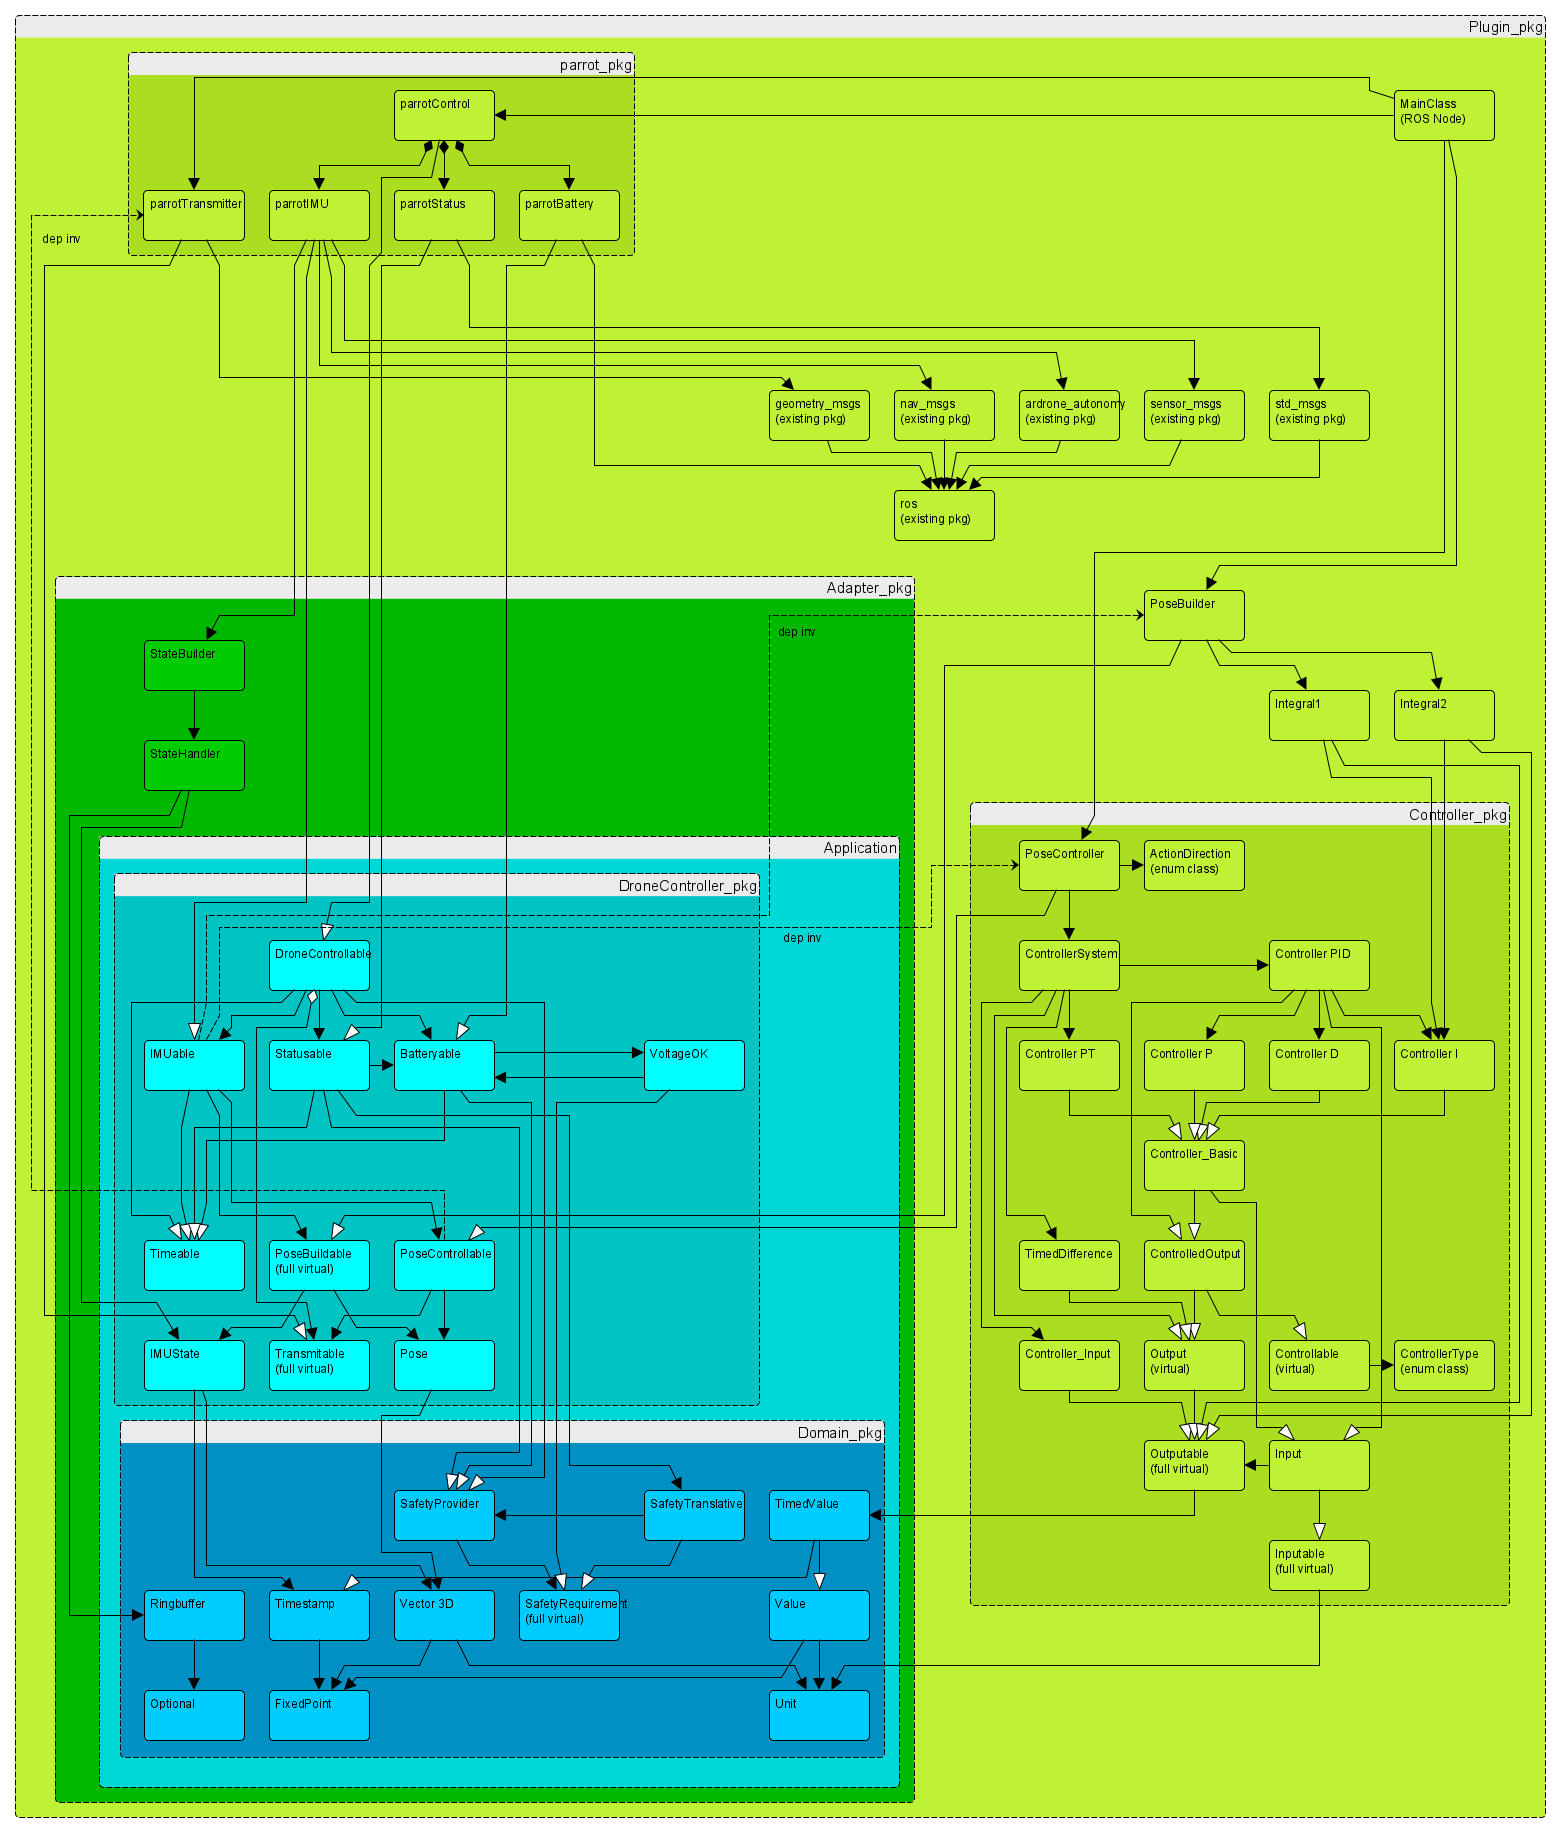
\includegraphics[height=20cm]{Pictures/Clean Architecture.png}}
\caption{Architektur des Positionsregelungssystems}
\label{fig:CArch}
\end{center}

\vspace{0.25cm}
\refImgShort{fig:CArch} zeigt die Architektur der Implementierung. Hierbei wurde die \clean\ zu Grunde gelegt.
\end{figure}









